% !TeX root = surprises.tex

\selectlanguage{hebrew}

\chapter{בניית מצולע משוכלל עם 
$17$
צלעות}
\label{c.heptadecagon}

%%%%%%%%%%%%%%%%%%%%%%%%%%%%%%%%%%%%%%%%%%%%%%%%%%%%%%%%%%%%%%%

פרק זה מציג את החישוב של 
\L{Gauss}
שהראה שניתן לבנות  באמצעות סרגל ומחוגה
\L{\textbf{heptadecagon}},
מצולע משוכלל עם 
$17$
צלעות.
נציג גם בניה של המצולע ובנוסף בניות של משולש משוכלל ומחומש משוכלל.
\section{בניה של מצולעים משוכללים}

\subsection{היסטוריה}
היוונים ידעו לבנות מצולעים משוכללים מסויימים  עם סרגל ומחוגה: משולש, ריבוע, מחומש ומצולע משוכלל עם $15$ צלעות.
כמובן, בהינתן מצולע משוכלל עם
$n$
צלעות, קל לבנות מצולע עם 
$2n$
צלעות על ידי בניית חוצי הצלעות.

לא הייתה התקדמות במשך אלפיים שנה עד שבשנת
$1796$,
קצת לפני יום הולדתו ה-$19$,
\L{Carl Friedrich Gauss}
התעורר בוקר אחד ולאחר "מחשבה מרוכזת" מצא דרך לבנות מצולע משוכלל עם 
$17$
צלעות. הישג זה עודד אותו להיות מתמטיקאי.

הבניה של מצולע משוכלל עם 
$17$
צלעות היתה אבן דרך למשפט
\L{Gauss-Wantzel}:
מצולע משוכלל עם 
$n$
צלעות ניתן לבנות עם סרגל ומחוגה אם ורק אם 
$n$
הוא מכפלה של חזקה של
$2$
ואפס או יותר מספרי 
\L{Fermat}
ראשונים
\textbf{שונים}
$2^{2^k}+1$.
מספרי 
\L{Fermat}
הראשונים הידועים הם:%
\footnote{%
\R{הוכח שעבור}
$5\leq k \leq 32$
\R{מספרי}
\L{Fermat}
\R{אינם ראשוניים}.}
\[
F_0=3,\: F_1=5,\: F_2=17,\: F_3=257,\: F_4=65537\,.
\]
מצולע משוכלל עם
$257$
צלעות נבנה לראשונה על ידי
\L{Magnus Georg Paucker}
ב-%
$1822$
ועל ידי
\L{Friedrich Julius Richelot}
ב-%
$1832$.
ב-%
$1894$
\L{Johann Gustav Hermes}
טען שבנה מצולע משוכלל עם
$65537$
צלעות.
כתב היד שלו נשמר באוניברסיטת 
\L{G\"{o}ttigen}.

נתון קטע קו שאורכו מוגדר כ-%
$1$,
האורכים שניתנים לבנייה הם אלה שניתן לקבל מאורכים קיימים תוך שימוש בפעולות 
$\{+,-,\times,/,\surd\}$.


\subsection{הקוסינוס של הזווית המרכזית}
כדי לבנות מצולע משוכלל מספיק לבנות קטע קו באורך 
$\cos \theta$,
כאשר
$\theta$ 
היא הזווית המרכזית במעגל היחידה עליה נשען המיתר שהוא צלע של המצולע. נתון קטע הקו
$\overline{OB}=\cos\theta$,
בנו אנך ב-%
$B$
וסמנו את החיתוך שלו עם מעגל היחידה ב-%
$C$.
אזי
$\overline{OC}=1$
ו-%
$\cos \theta=\disfrac{\overline{OB}}{\overline{OC}}=\overline{OB}$.
המיתר 
$\overline{AC}$
הוא צלע של המצולע.

\begin{center}

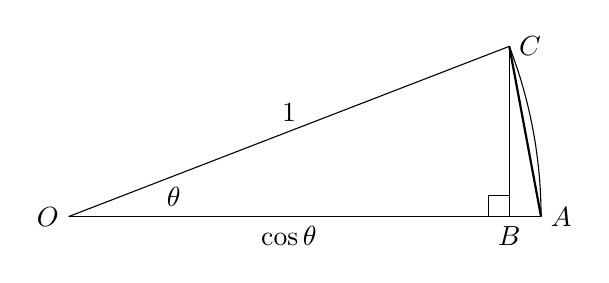
\begin{tikzpicture}[scale=1.5]
\coordinate (O) at (0,0) node[left] {$O$} node[above right,xshift=32pt] {$\theta$};
\coordinate (A) at (4,0);
\node[right] at (A) {$A$};
\draw (O) -- (A);
\draw (A) arc(0:21.12:4);
\coordinate (C) at (21.12:4cm);
\draw (O) -- node[above] {$1$} (C);
\node[right] at (C) {$C$};
\draw (C) -- (C |- A) coordinate (B);
\node[below] at (B) {$B$};
\draw[rotate=90] (B) rectangle +(5pt,5pt);
\draw[thick] (A) -- (C);
\path (O) -- node[below] {$\cos \theta$} (B); 
\end{tikzpicture}
\end{center}
הזווית המרכזית של מצולע משוכלל עם 
$17$
צלעות היא
$\disfrac{2\pi}{17}$
רדיאנים או
$\disfrac{360^\circ}{17}\approx 21.12^\circ$. 
\begin{center}

\begin{tikzpicture}[scale=1]
\coordinate (O) at (0,0);
\foreach \x/\name in {0/a,1/b,2/c,3/d,4/e,5/f,6/g,7/h,8/i,9/j,10/k,11/l,12/m,13/n,14/o,15/p,16/q} {
  \coordinate (\name) at ($(O)+(\x*21.12:3cm)$);
  \draw (O) -- (\name);
  \fill (\name) circle (1pt);
}
\draw (a) -- (b) -- (c) -- (d) -- (e) -- (f) -- (g) -- (h) -- (i) -- (j) -- (k) -- (l) -- (m) -- (n) -- (o) -- (p) -- (q) -- cycle;
\node[above right,xshift=39pt] at (O) {$2\pi/17=21.12^\circ$};
\draw (O) circle (3cm);
\end{tikzpicture}
\end{center}
\L{Gauss}
הראה ש:

\begin{eqn}
\cos\left(\disfrac{2\pi}{17}\right) &=& 
-\disfrac{1}{16}+\disfrac{1}{16}\sqrt{17} + 
     \disfrac{1}{16}\sqrt{34-2\sqrt{17}}
    + \\
    &&
     \disfrac{1}{8}\sqrt{
     17+3\sqrt{17} - 
     \sqrt{34-2\sqrt{17}}
   -2
     \sqrt{34+2\sqrt{17}}
   }\,.
\end{eqn}
ערך זה ניתן לחשב תוך שימוש בפעולות
$\{+,-,\times,/,\surd\}$
ולכן ניתן לבנות את המצולע.

%%%%%%%%%%%%%%%%%%%%%%%%%%%%%%%%%%%%%%%%%%%%%%%%%%%%%%

\section{המשפט הבסיסי של אלגברה}

נשתמש במשפט שלהלן ללא הוכחה:
\begin{theorem}[\R{המשפט הבסיסי של אלגברה}]\label{thm.fundamental}\mbox{}\\
לכל פולינום ממעלה 
$n$
)עם מקדמים מרוכבים(
יש בדיוק
$n$
שורשים
)מרוכבים(.
\end{theorem}


%%%%%%%%%%%%%%%%%%%%%%%%%%%%%%%%%%%%%%%%%%%%%%%%%%%%%%

\section{שורשי היחידה}\label{s.roots}

נתבונן במשוואה
$x^{n}-1=0$
עבור כל מספר שלם
$n>	 1$.
שורש אחד הוא
$x=1$.
לפי משפט~%
\ref{thm.fundamental}
קיימים
$n-1$
שורשים נוספים. נסמן שורש אחד מתוכם ב-%
$r$
כך ש-%
$r^{n}=1$.
$r$
נקרא

נתבונן כעת ב-%
$r^2$.
אנו רואים ש:
\[
(r^2)^n=(r^{n})^2=1^2=1\,.
\]
חישוב דומה עבור כל חזקה של
$r$
מראה שכל החזקות הם שורשי היחידה:
\[
1, r, r^2, \ldots, r^{n-2}, r^{n-1}\,.
\]



\begin{theorem}\label{thm.roots-of-unity}\mbox{}\\
יהי
$n$
ראשוני ו-%
$r$
שורש היחידה מסדר 
$n$.
אזי
$\{1,r,r^2,\ldots,r^{n-2},r^{n-1}\}$
שונים זה מזה ולכן הם מהווים את 
\textbf{כל}
שורשי היחידה מסדר
$n$.
\end{theorem}
\textbf{הוכחה:}
נניח ש-%
$r^i=r^j$
עבור מספרים כלשהם
$1\leq i<j\leq n$.
$r^j/r^i=r^{j-i}=1$,
כלומר, קיים מספר
$m$,
$m<n$
כך ש-%
$r^m=1$.
נניח ש-%
$m$
הוא המספר הקטן ביותר עם תכונה זו. 
לפי חילוק של שלמים עם שארית,
$n=ml+k$
עבור
$0<l<n$,
$0\leq k<m$:
\[
1=r^n=r^{ml+k}=(r^m)^l\cdot r^k=1^l\cdot r^k=r^k\,,
\]
ולכן 
$0\leq k<m$ 
ו-%
$r^k=1$,
סתירה להנחה ש-%
$m$
הוא המספר הקטן ביותר המקיים את התנאי. מכאן ש-%
$k=0$
ו-%
$n=ml$,
כך ש-%
$n$
אינו ראשוני.
\qed

נשתמש במשפט שלהלן ללא הוכחה:
\begin{theorem}\mbox{}\\
יהיו
$\{a_1,a_2,\ldots,a_{n-1},a_n\}$
השורשים של פולינום
$f(x)$
מסדר
$n$.
אזי:
\[
f(x) =(x-a_1) (x-a_2)\cdots (x-a_{n-1})(x-a_n)\,.
\]
\end{theorem}



מהנוסחה של
\L{Viet\'{e}}
)עמוד~%
$82$ 
של
\L{\cite{jorg}}(
מתקבלים המקדמים של הפולינום כביטויים עם השורשים. עבור
$x^{n-1}$
המקדם הוא:
\[
-(a_1+a_2+\cdots+a_{n-1}+a_n)\,.
\]
בפולינום
$x^n-1$,
ברור שהמקדם של 
$x^{n-1}$
הוא אפס ולכן:
\[
1+r+r^2+\cdots + r^{n-2}+r^{n-1}=0\,.
\]
נשמתמש בעובדה זו בצורה:
\[
r+r^2+\cdots + r^{n-2}+r^{n-1}=-1\,.
\]
עבור מצולע משוכלל עם 
$17$
צלעות המשוואה היא:
\[
r+r^2+r^3+r^4+r^5+r^6+r^7+r^8+r^9+r^{10}+r^{11}+r^{12}+r^{13}+r^{14} + r^{15}+r^{16}=-1\,,
\]

\section{ההוכחה של 
\L{Gauss}
שניתן לבנות 
\L{heptadecagon}}\label{s.gauss}

אין חובה לעבוד עם השורשים בסדר הטבעי שלהם
$r,r^2,\ldots,r^{16}$. 
החזקות של
$r^3$
נותנות אם כל השורשים אבל בסדר שונה. עבור
$k<17$, $r^{17m+k}=(r^{17})^m\cdot r^k=1^m\cdot r^k=r^k$,
ולכן רשמנו את החזקות כשאריות לאחר חלוקה ב-%
$17$.

\begin{eqnlabels}
r^1, \;r^{1\cdot 3 =3},\; r^{3\cdot 3=9},\; r^{9\cdot 3=27=10},\; r^{10\cdot 3=30=13},\; r^{13\cdot 3=39=5},\; r^{5\cdot 3=15},\; r^{15\cdot 3=45=11},\\
r^{11\cdot 3 =33=16}, \;r^{16\cdot 3=48=14},\; r^{14\cdot 3=42=8},\; r^{8\cdot 3=24=7},\;r^{7\cdot 3=21=4},\; r^{4\cdot 3=12},\; r^{12\cdot 3=36=2},\; r^{2\cdot 3=6}\,.
\end{eqnlabels}



חשוב שתבדקו שהרשימה כוללת את כל 
$16$
השורשים בדיוק פעם אחת.

המטרה של
\L{Gauss}
היתה למצוא את ערך השורש
$r$
על ידי פתרון של משוואות ריבועיות, כך שניתן לבנות אותו עם סרגל ומחוגה. נתבונן במשוואה הריבועית:
\[
x^2+px+q=0\,,
\]
ונניח שהשורשים שלה הם:
$a,b$.
אזי:
\[
(x-a)(x-b)=x^2 - (a+b)x + ab\,.
\]
לכן
$p=-(a+b)$
ו-%
$q=ab$.

אם
\textbf{נתונים}
$a+b$
ו-%
$ab$,
נוכל לרשום את המשוואה הריבועית עבורה הם השורשים.%
\footnote{\R{ראו פרק}
\ref{c.quadratic}
\R{המציג שיטה למציאת שורשים של משוואה ריבועית המבוססת על הרעיון הזה}.}

יהי
$a_0$
החיבור של השורשים במקומות האי-זוגיים ברשימה לעיל:
\[
a_0=r + r^9 + r^{13} +r^{15} +r^{16} + r^8+r^4+r^2\,,
\]
ויהי
$a_1$
הסכום של השורשים במקומות הזוגיים ברשימה:
\[
a_1=r^3 + r^{10} + r^{5} +r^{11} +r^{14} + r^7+r^{12}+r^6\,.
\]
כדי לקבל את
$a_0,a_1$
כשורשים של משוואה ריבועית, תחילה נחשב את הסכום שלהם:
\[
a_0+a_1=r + r^2 + \cdots +r^{16}=-1\,.
\]
כדי למצוא את המשוואה הריבועית עלינו לחשב את
$a_0a_1$.
החישוב מעט מסורבל ומוצג באיור%
~\ref{fig.a0a1}.
הערכים של
$r^ir^j$
רשומים לאחר חישוב
$r^{(i+j) \bmod 17}$.
מתחת לכל שורש נמצא מספר המופעים שלו עד כה;
בדקו שכל שורש מופיע בדיוק ארבע פעמיים כך שערכה של המכפלה הוא 
$-4$.
\begin{figure}[tb]
\begin{eqn}
a_0a_1&=&(r + r^9 + r^{13} +r^{15} +r^{16} + r^8+r^4+r^2)\;\cdot\\
&&(r^3 + r^{10} + r^{5} +r^{11} +r^{14} + r^7+r^{12}+r^6)\\
&=&\occ{4}{1} + \occ{11}{1} + \occ{6}{1} + \occ{12}{1} + \occ{15}{1} + \occ{8}{1} + \occ{13}{1} + \occ{7}{1} +\\
&&\occ{12}{2} + \occ{2}{1} + \occ{14}{1} + \occ{3}{1} + \occ{6}{2} + \occ{16}{1} + \occ{4}{2} + \occ{15}{2} +\\
&&\occ{16}{2} + \occ{6}{3} + \occ{1}{1} + \occ{7}{2} + \occ{10}{1} + \occ{3}{2} + \occ{8}{2} + \occ{2}{2}\;\;\: +\\
&&\occ{1}{2} + \occ{8}{3} + \occ{3}{3} + \occ{9}{1} + \occ{12}{3} + \occ{5}{1} + \occ{10}{2} + \occ{4}{3}\;\;\: +\\
&&\occ{2}{3} + \occ{9}{2} + \occ{4}{4} + \occ{10}{3} + \occ{13}{2} + \occ{6}{4} + \occ{11}{2} + \occ{5}{2} \:+\\
&&\occ{11}{3} + \occ{1}{3} + \occ{13}{3} + \occ{2}{4} + \occ{5}{2} + \occ{15}{3} + \occ{3}{4} + \occ{14}{2} \;+\\
&&\occ{7}{3} + \occ{14}{3} + \occ{9}{3} + \occ{15}{4} + \occ{1}{4} + \occ{11}{4} + \occ{16}{3} + \occ{10}{4} +\\
&&\occ{5}{4} + \occ{12}{4} + \occ{7}{4} + \occ{13}{4} + \occ{16}{4} + \occ{9}{4} + \occ{14}{4} + \occ{8}{4}\\
&=&-4\,.
\end{eqn}
\selectlanguage{hebrew}
\caption{החישוב של $a_0a_1$}\label{fig.a0a1}
\end{figure}

מ-%
$a_0\!+\!a_1\!=\!-1$
ו-%
$a_0,a_1\!=\!-4$,
אנו יודעים ש-%
$a_0,a_1$
הם השורשים של המשוואה:
\[
x^2+x-4=0\,.
\]
השורשים הם:
\[
a_{0,1} = \frac{-1\pm\sqrt{17}}{2}\,.
\]



יהי
$b_0,b_1,b_2,b_3$
הסכום של כל שורש רביעי החל מ-%
$r^1,r^3,r^9,r^{10}$,
בהתאמה:

\begin{eqn}
b_0&=& r^1+ r^{13} + r^{16} + r^4\\
b_1&=& r^3+ r^{5} + r^{14} + r^{12}\\
b_2&=& r^9+ r^{15} + r^{8} + r^2\\
b_3&=& r^{10}+ r^{11} + r^{7} + r^6\,.
\end{eqn}
בדקו ש-%
$b_0+b_2=a_0, b_1+b_3=a_1$
)איורים~%
\ref{f.b0b2}, \ref{f.b1b3}(.
\begin{figure}

\begin{eqn}
b_0b_2&=&(r + r^{13} + r^{16} +r^4)\;\times\\
&&(r^9 + r^{15} + r^{8} +r^{2})\\
&=& r^{10}+r^{16}+r^9+r^3+\\
&& r^{5}+r^{11}+r^4+r^{15}+\\
&& r^{8}+r^{14}+r^7+r^1\;\:+\\
&& r^{13}+r^{2}+r^{12}+r^6\\
&=&-1\,.
\end{eqn}
\selectlanguage{hebrew}
\caption{החישוב של $b_0b_2$}\label{f.b0b2}
\end{figure}
\begin{figure}

\begin{eqn}
b_1b_3&=&(r^3 + r^{5} + r^{14} +r^{12})\times\\
&&(r^{10} + r^{11} + r^{7} +r^{6})\\
&=& r^{13}+r^{14}+r^{10}+r^9\;+\\
&& r^{15}+r^{16}+r^{12}+r^{11}+\\
&& r^{7}+r^{8}+r^4+r^3\quad\;\;+\\
&& r^{5}+r^{6}+r^{2}+r^1\\
&=&-1\,.
\end{eqn}
\selectlanguage{hebrew}
\caption{החישוב של $b_1b_3$}\label{f.b1b3}
\end{figure}

נסכם את החישובים:

\begin{eqn}
b_0+b_2&=&a_0\\
b_0b_2&=&-1\\
b_1+b_3&=&a_1\\
b_1b_3&=&-1\,.
\end{eqn}



$b_0,b_2$ 
הם השורשים של:
\[
x^2-a_0x-1= 0\,,\\
\]
ו-%
$b_1,b_3$
הם השורשים של:
\[
x^2-a_1x-1 =0\,.
\]
מהנוסחה לפתרון משוואות ריבועיות ומהערכים שחישבנו קודם עבור 
$a_0,a_1$,
מתקבלים השורשים
$b_0,b_1$
)איור~%
\ref{fig.b0}, \ref{fig.b1}(.
\begin{figure}[tb]

\begin{eqn}
b_0&=&\disfrac{a_0+\sqrt{a_0^2+4}}{2}\\
&=&\disfrac{
     \disfrac{(-1+\sqrt{17})}{2} + 
     \sqrt{\left[\disfrac{(-1+\sqrt{17})}{2}\right]^2+4}
   }{2}\\
&=&\disfrac{
     (-1+\sqrt{17}) + 
     \sqrt{\left[-1+\sqrt{17}\right]^2+16}
   }{4}\\
&=&\disfrac{
     (-1+\sqrt{17}) + 
     \sqrt{34-2\sqrt{17}}
   }{4}\,,
\end{eqn}%
\caption{\R{החישוב של} $b_0$}\label{fig.b0}
\end{figure}
\begin{figure}

\begin{eqn}
b_1&=&\disfrac{a_1+\sqrt{a_1^2+4}}{2}\\
&=&\disfrac{
     \disfrac{(-1-\sqrt{17})}{2} + 
     \sqrt{\left[\disfrac{(-1-\sqrt{17})}{2}\right]^2+4}
   }{2}\\
&=&\disfrac{
     (-1-\sqrt{17}) + 
     \sqrt{\left[-1-\sqrt{17}\right]^2+16}
   }{4}\\
&=&\disfrac{
     (-1-\sqrt{17}) + 
     \sqrt{34+2\sqrt{17}}
   }{4}\,.
\end{eqn}
\selectlanguage{hebrew}
\caption{החישוב של $b_1$}\label{fig.b1}
\end{figure}
לבסוף יהי
$c_0,c_4$ 
הסכום של כל שורש שמיני החל מ-%
$r^1,r^{13}$,
בהתאמה:%
\footnote{\R{יש סכומים נוספים אבל שני אלה יספיקו}.}

\begin{eqn}
c_0&=&r^1+r^{16}\\
c_4&=&r^{13}+r^4\\
c_0+c_4&=&r^1+r^{16}+r^{13}+r^4=b_0\\
c_0c_4&=&(r^1+r^{16})\cdot(r^{13}+r^4)\\
&=&r^{14}+r^5+r^{12}+r^3=b_1\,.
\end{eqn}

$c_0,c_4$
הם השורשים של:
\[
y^2-b_0y+b_1=0\,.
\]
נראה שמספיק לחשב את השורש
$c_0=r^1+r^{16}$
)איור~
\ref{fig.c0}(.

\begin{figure}

\begin{eqn}
c_0&=&\disfrac{b_0+\sqrt{b_0^2-4b_1}}{2}\\
&=&\disfrac{
     \disfrac{
     (-1+\sqrt{17}) +
     \sqrt{34-2\sqrt{17}}
   }{4}}{2} + \\
&& 
    \disfrac{
       \sqrt{\left[\disfrac{
     (-1+\sqrt{17}) + 
     \sqrt{34-2\sqrt{17}}
   }{4}\right]^2-4\left[\disfrac{
     (-1-\sqrt{17}) + 
     \sqrt{34+2\sqrt{17}}
   }{4}\right]}
   }{2}\\
&=&-\disfrac{1}{8}+\disfrac{1}{8}\sqrt{17} + 
     \disfrac{1}{8}\sqrt{34-2\sqrt{17}}
    + \\
   &&
     \disfrac{1}{8}\sqrt{
     \left[
     (-1+\sqrt{17}) + 
     \sqrt{34-2\sqrt{17}}
   \right]^2-16\left[
     (-1-\sqrt{17}) + 
     \sqrt{34+2\sqrt{17}}
   \right]}
\\
&=&-\disfrac{1}{8}+\disfrac{1}{8}\sqrt{17} + 
     \disfrac{1}{8}\sqrt{34-2\sqrt{17}}
    + \\
   &&
     \disfrac{1}{8}\sqrt{
     (-1+\sqrt{17})^2 + 
     2(-1+\sqrt{17})\sqrt{34-2\sqrt{17}}+
     (34-2\sqrt{17})
   -}\\
   &&\overline{
     \left[(-16-16\sqrt{17}) + 
     16\sqrt{34+2\sqrt{17}}\right]
   }
\\
&=&-\disfrac{1}{8}+\disfrac{1}{8}\sqrt{17} + 
     \disfrac{1}{8}\sqrt{34-2\sqrt{17}}
    + \\
   &&
     \disfrac{1}{8}\sqrt{
     68+12\sqrt{17} + 
     2(-1+\sqrt{17})\sqrt{34-2\sqrt{17}}
   -16
     \sqrt{34+2\sqrt{17}}
   }
\end{eqn}
\selectlanguage{hebrew}
\caption{החישוב של $c_0$}\label{fig.c0}
\end{figure}

\clearpage

סיימנו כי:
\[
c_0=r_1+r_{16}=2\cos\left(\frac{2\pi}{17}\right)\,.
\]
קואורדינטות ה-%
$y$
של
$r_1,r_{16}$
שוות עם סימנים הפוכים ולכן הסכום שלהם אפס. קואורדינטות ה-%
$x$
נספרות פעמיים:
%\begin{figure}
\begin{center}

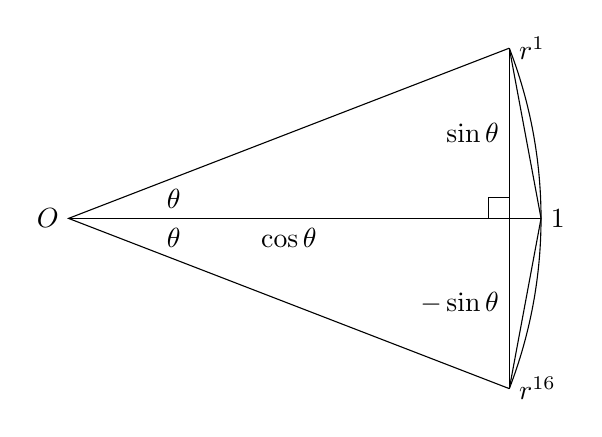
\begin{tikzpicture}[scale=1.5]
\coordinate (O) at (0,0) node[left] {$O$} node[above right,xshift=32pt] {$\theta$} node[below right,xshift=32pt] {$\theta$};
\coordinate (A) at (4,0);
\node[right] at (A) {$1$};
\draw (O) -- (A);
\coordinate (C) at (21.12:4cm);
\coordinate (D) at (-21.12:4cm);
\draw (D) arc(-21.12:21.12:4);
\draw (D) -- (O) -- (C);
\node[right] at (C) {$r^1$};
\node[right] at (D) {$r^{16}$};
\draw (C) -- (C |- A) coordinate (B);
\draw (D) -- (D |- A);
%\node[below left] at (B) {$B$};
\draw[rotate=90] (B) rectangle +(5pt,5pt);
\draw (D) -- node[left,xshift=-6pt] {$-\sin\theta$} (A) -- node[left,xshift=-6pt] {$\sin \theta$} (C);
\path (O) -- node[below] {$\cos \theta$} (B);
\end{tikzpicture}
%\caption{בניית צלע מהזווית המרכזית שהוא כולא}\label{fig.two-cosine}
\end{center}
%\end{figure}


הוכחנו שניתן לבנות קטע קו באורך הקוסינוס של הזווית המרכזית של מצולע משוכלל עם 
$17$
צלעות, כי הוא מורכב רק ממספרים רציונליים והפעולות 
$\{+,-,\times,/,\surd\}$:

\begin{eqn}
\cos\left(\disfrac{2\pi}{17}\right) &=& 
-\disfrac{1}{16}+\disfrac{1}{16}\sqrt{17} + 
     \disfrac{1}{16}\sqrt{34-2\sqrt{17}}
    + \\
    &&
     \disfrac{1}{16}\sqrt{
     68+12\sqrt{17} + 
     2(-1+\sqrt{17})\sqrt{34-2\sqrt{17}}
   -16
     \sqrt{34+2\sqrt{17}}
   }
\end{eqn}

נסכם את הייצוג של השורשים של
$x^{17}-1$
כמספרים מרוכבים.%
\footnote{%
מספרים מרוכבים עומדים במרכז החקר של השורשים של פולינומים. קוראים שלא מכירים את הנושא יכולים לדלג על סעיף זה.}

השורש
$r$
של
$x^n-1$
הוא
\[
\cos \left(\disfrac{2\pi}{n}\right) + i\sin  \left(\disfrac{2\pi}{n}\right)\,,
\]
כי לפי נוסחאת
\L{de Moivre}:
\[
\left[\cos \left(\disfrac{2\pi}{n}\right) + i\sin  \left(\disfrac{2\pi}{n}\right)\right]^{n}=
\cos \left(\disfrac{2\cdot n\pi}{n}\right) + i\sin  \left(\disfrac{2\cdot n\pi}{n}\right)= 1\,,
\]
הקשר בין 
$c_0$
לבין הקוסינוס של הזווית המרכזית של המצולע מתקבל בקלות:
\begin{eqn}
c_0&=&r_1+r_{16}\\
&=&\left[\cos\left(\disfrac{2\pi}{17}\right)+i\sin\left(\disfrac{2\pi}{17}\right)\right]+\left[\cos\left(\disfrac{2\cdot 16\pi}{17}\right)+i\sin\left(\disfrac{2\cdot 16\pi}{17}\right)\right]\\
&=&\left[\cos\left(\disfrac{2\pi}{17}\right)+\cos\left(\disfrac{-2\pi}{17}\right)\right]+i\left[\sin\left(\disfrac{2\pi}{17}\right)+\sin\left(\disfrac{-2\pi}{17}\right)\right]\\
&=&2\cos\left(\disfrac{2\pi}{17}\right)+i\cdot 0=2\cos\left(\disfrac{2\pi}{17}\right)\,.
\end{eqn}

%%%%%%%%%%%%%%%%%%%%%%%%%%%%%%%%%%%%

\section{פיתוח הנוסחה של %
\L{Gauss}%
}\label{s.derivation}

הנוסחה שקיבלנו עבור 
$\cos\left(\disfrac{2\pi}{17}\right)$
איננה הנוסחה שניתנה על ידי
\L{Gauss}
עצמו
)ראו עמוד
$458$
של
\L{\cite{gauss}}
ועמוד
$68$
של
\L{\cite{jorg}}(.
את הנוסחה שקיבלתי מצאתי רק ב-%
\L{\cite{rike}}
ביחד עם תרגיל להמיר אותה לנוסחה של
\L{Gauss}.
סעיף זה פותר את התרגיל.

נפשט את הביטוי
$2(-1+\sqrt{17})\sqrt{34-2\sqrt{17}}$:

\begin{eqn}
2(-1+\sqrt{17})\sqrt{34-2\sqrt{17}} &=&
-2\sqrt{34-2\sqrt{17}} +2\sqrt{17}\sqrt{34-2\sqrt{17}}+\\
&&4\sqrt{34-2\sqrt{17}}-4\sqrt{34-2\sqrt{17}}\\
&=&
2\sqrt{34-2\sqrt{17}} +2\sqrt{17}\sqrt{34-2\sqrt{17}}+\\
&&-4\sqrt{34-2\sqrt{17}}\\
%&=&\left(-2\sqrt{34-2\sqrt{17}} +2\sqrt{17}\sqrt{34-2\sqrt{17}}
%+4\sqrt{34-2\sqrt{17}}\right)\\
%&&-4\sqrt{34-2\sqrt{17}}\\
&=&2(1+\sqrt{17})\sqrt{34-2\sqrt{17}}-4\sqrt{34-2\sqrt{17}}\,.
\end{eqn}
נזכור את הביטוי
$-4\sqrt{34-2\sqrt{17}}$
ונפשט את הביטוי הראשון. נרבע אותו ואז נוציא שורש הריבועי:

\begin{eqn}
2(1+\sqrt{17})\sqrt{34-2\sqrt{17}}&=&
2\sqrt{\left[(1+\sqrt{17})\sqrt{34-2\sqrt{17}}\right]^2}\\
&=&2\sqrt{(18+2\sqrt{17})(34-2\sqrt{17})}\\
&=&2\sqrt{(18\cdot 34-4\cdot17)+\sqrt{17}(2\cdot 34 - 2\cdot 18)}\\
&=&2\cdot 4\sqrt{34+2\sqrt{17}}\,.
\end{eqn}
נציב את הביטויים ונקבל את הנוסחה של \L{Gauss}:

\begin{eqn}
\cos\left(\disfrac{2\pi}{17}\right) &=& 
-\disfrac{1}{16}+\disfrac{1}{16}\sqrt{17} + 
     \disfrac{1}{16}\sqrt{34-2\sqrt{17}}
    + \\
    &&
     \disfrac{1}{16}\sqrt{
     68+12\sqrt{17} + 
     2\cdot 4\sqrt{34+2\sqrt{17}}-4\sqrt{34-2\sqrt{17}}
   -16
     \sqrt{34+2\sqrt{17}}
   }\\
&=&-\disfrac{1}{16}+\frac{1}{16}\sqrt{17} + 
     \disfrac{1}{16}\sqrt{34-2\sqrt{17}}
    + \\
    &&
     \disfrac{1}{8}\sqrt{
     17+3\sqrt{17} - 
     \sqrt{34-2\sqrt{17}}
   -2
     \sqrt{34+2\sqrt{17}}
   }
\end{eqn}


\section{בניית
\L{heptadecagon}
עם סרגל ומחוגה}
\label{s.construction}

בנו מעגל יחידה שמרכזו
$O$,
עם קוטרים ניצבים
$\overline{PQ},\overline{RS}$.
\begin{center}

\begin{tikzpicture}[scale=1.5]
\clip (-5,-1.8) rectangle (5,1.8);

\node at (-.2,1.5) {$\cdots$};
\node at (-.2,1.7) {$R$};
\node at (-.2,-1.5) {$\cdots$};
\node at (-.2,-1.7) {$S$};

\coordinate (O) at (0,0);
\draw (O) circle (4cm);
\coordinate (P) at (4,0);
\coordinate (R) at (0,4);
\coordinate (Q) at (-4,0);
\coordinate (S) at (0,-4);
\coordinate (A) at (0,1);
\coordinate (B) at (.78,0);
\coordinate (C) at (-1.28,0);
\draw (P) -- (Q);
\draw (R) -- (S);
\path (O) -- node[left,xshift=2pt,yshift=-4pt] {\sm{\frac{1}{4}}} (A);
\draw[dashed] (P) -- ($(P)!1.5!(A)$);
\draw (A) -- node[above] {$\frac{\sqrt{17}}{4}$} (P);
\draw (C) -- (A) -- (B);
\foreach \c/\where in {O/below left, P/right, Q/left, R/above, S/below, A/above left, B/below, C/below} {
  \fill (\c) circle(1pt) node[\where] {$\c$};
}
\draw (O) rectangle(+6pt,+6pt);
\node[below right,xshift=8pt,yshift=-4pt] at (A) {\sm{\alpha}};
\node[below right,xshift=-3pt,yshift=-4pt] at (A) {\sm{\alpha}};
\node[below left,xshift=1pt,yshift=-2pt] at (A) {\sm{\beta}};
\node[below left,xshift=-4pt,yshift=4pt] at (A) {\sm{\beta}};
\draw[<->] ($(C)+(0,-16pt)$) -- node[below] {\sm{\frac{1+\sqrt{17}}{16}}} ($(O)+(0,-16pt)$);
\draw[<->] ($(O)+(0,-16pt)$) -- node[below,xshift=4pt] {
\sm{
\frac{-1+\sqrt{17}}{2}
}
} ($(B)+(0,-16pt)$);
\end{tikzpicture}
\end{center}
בנו נקודה
$A$
כך ש-%
$\overline{OA}=\disfrac{1}{4}\overline{OR}$.
לפי משפט פיתגורס,
$\overline{AP}=\sqrt{(1/4)^2+1^2}=\sqrt{17}/4$.

יהי
$B$
נקודת החיתוך של 
$\angle OAP$
עם ציר ה-%
$x$,
ויהי 
$C$
נקודת החיתוך של הזווית המשלימה ל-%
$\angle OAP$ 
עם ציר ה-%
$x$.
לפי משפט חוצה הזווית
\L{\cite{wiki:bisector}}:

\begin{eqn}
\disfrac{\overline{OB}}{\overline{BP}}&=&\disfrac{\overline{AO}}{\overline{AP}}\\
\disfrac{\overline{OB}}{1-\overline{OB}}&=&\disfrac{1/4}{\sqrt{17}/{4}}\\
\overline{OB}&=&\disfrac{1}{1+\sqrt{17}}=\disfrac{1}{1+\sqrt{17}}\cdot \disfrac{1-\sqrt{17}}{1-\sqrt{17}}\\
&=&\disfrac{-1+\sqrt{17}}{16}\,,
\end{eqn}



ו:

\begin{eqn}
\disfrac{\overline{OC}}{\overline{CP}}&=&\disfrac{\overline{AO}}{\overline{AP}}\\
\disfrac{\overline{OC}}{1+\overline{OC}}&=&\disfrac{1/4}{\sqrt{17}/{4}}\\
\overline{OC}&=&\disfrac{1}{-1+\sqrt{17}}=\disfrac{1}{-1+\sqrt{17}}\cdot \disfrac{1+\sqrt{17}}{1+\sqrt{17}}\\
&=&\disfrac{1+\sqrt{17}}{16}\,.
\end{eqn}
בנו
$D$
על
$\overline{OP}$
כך ש-%
$\overline{CD}=\overline{CA}$:
\begin{center}

\begin{tikzpicture}[scale=1.5]
\clip (-5,-1.5) rectangle (5,1.5);
\coordinate (O) at (0,0);
\draw (O) circle (4cm);
\coordinate (P) at (4,0);
\coordinate (R) at (0,4);
\coordinate (Q) at (-4,0);
\coordinate (S) at (0,-4);
\coordinate (A) at (0,1);
\coordinate (B) at (.78,0);
\coordinate (C) at (-1.28,0);

\coordinate (D) at (.344,0);
\coordinate (E) at (2.05,0);
\coordinate (M) at (-1.8275,0);
\coordinate (F) at (0,-1);

\draw (P) -- (Q);
\draw (R) -- (S);
\draw (A) -- (P);
\draw (C) -- node[above] {$a$} (A) -- node[above,xshift=2pt] {$b$} (B);
\path (Q) -- node[below] {$f$}  (M);
\path (B) -- node[below] {$b$} (E);

\path[name path=circ] (M) circle (2.1725cm);
\path[name path=yaxis] (R) -- (S);
\path[name intersections={of=circ and yaxis,by={F1,F}}];
\draw (M) -- node[below] {$f$} (F);

\draw[<->] ($(C)+(0,-15pt)$) -- node[fill=white] {$a$} ($(D)+(0,-15pt)$);

\foreach \c/\where in {O/below left, P/right, Q/left, R/above, S/below, A/above left, B/below, C/below, D/below, E/below, M/below left, F/below left} {
  \fill (\c) circle(1pt) node[\where] {$\c$};
}
\draw (O) rectangle(+6pt,+6pt);
\end{tikzpicture}
\end{center}

\begin{eqn}
\overline{CD}=\overline{CA}&=&\sqrt{\overline{OA}^2+\overline{OC}^2}\\
&=&\sqrt{\left(\disfrac{1}{4}\right)^2+\left(\disfrac{1+\sqrt{17}}{16}\right)^2}\\
&=&\disfrac{1}{16}\sqrt{34+2\sqrt{17}}\,.
\end{eqn}
בנו
$E$
על
$\overline{OP}$
כך ש-%
$\overline{BE}=\overline{BA}$:

\begin{eqn}
\overline{BE}=\overline{BA}&=&\sqrt{\overline{OA}^2+\overline{OB}^2}\\
&=&\sqrt{\left(\disfrac{1}{4}\right)^2+\left(\disfrac{1-\sqrt{17}}{16}\right)^2}\\
&=&\disfrac{1}{16}\sqrt{34-2\sqrt{17}}\,.
\end{eqn}


בנו
$M$,
נקודת האמצע של
$\overline{QD}$
ובנו
$F$
על
$\overline{OS}$
כך ש-%
$\overline{MF}=\overline{MQ}$:

\begin{eqn}
\overline{MF}=\overline{MQ}&=&\disfrac{1}{2}\overline{QD}=\disfrac{1}{2}(\overline{QC}+\overline{CD})=\disfrac{1}{2}((1-\overline{OC})+\overline{CD})\\
&=&\disfrac{1}{2}\left[1-\left(\disfrac{1+\sqrt{17}}{16}\right)+\disfrac{\sqrt{34+2\sqrt{17}}}{16}\right]\\
&=&\disfrac{1}{32}\left(15-\sqrt{17}+\sqrt{34+2\sqrt{17}}\right)\,.
\end{eqn}
בנו מעגל שקוטרו 
$\overline{OE}$.
בנו מיתר
$\overline{OG}=\overline{OF}$.
שימו לב ש-%
$\overline{MO}=1-\overline{MQ}=1-\overline{MF}$:



\begin{center}

\begin{tikzpicture}[scale=1.5]
\clip (-5,-1.5) rectangle (5,1.5);
\coordinate (O) at (0,0);
\draw (O) circle (4cm);
\coordinate (P) at (4,0);
\coordinate (R) at (0,4);
\coordinate (Q) at (-4,0);
\coordinate (S) at (0,-4);
\coordinate (A) at (0,1);
\coordinate (B) at (.78,0);
\coordinate (C) at (-1.28,0);

\coordinate (D) at (.5,0);
\coordinate (E) at (2.045,0);
\coordinate (M) at (-1.8275,0);

\path[name path=circ] (M) circle (2.1725cm);
\path[name path=yaxis] (R) -- (S);
\path[name intersections={of=circ and yaxis,by={F1,F}}];
\draw (M) -- node[below] {$f$} (F);

\draw[name path=OEarc,thick,dashed] (E) arc(0:-180:1.025cm);
\path[name path=OFcircle] (O)
  let
    \p1 = ($(O)-(F)$)
  in
    circle({veclen(\x1,\y1)});
\path[name intersections={of=OEarc and OFcircle, by={G}}];
\draw (O) -- node[above,near end,xshift=2pt] {$g$} (G) -- node[below] {$e$} (E);
\path (O) -- node[left] {$g$} (F);

\path[name path=EGcircle] (E) 
  let
  \p1 = ($(E)-(G)$)
  in
    circle({veclen(\x1,\y1)});
\draw[name path=PQ] (P) -- (Q);
\path[name intersections={of=PQ and EGcircle, by={H,H1}}];
\path (E) -- node[below] {$e$} (H);

\draw (R) -- (S);
\draw (A) -- (P);
\draw (C) -- (A) -- (B);
\draw (M) -- (F);

\foreach \c/\where in {O/below left, P/right, Q/left, R/above, S/below, A/above left, B/below, C/below, D/below, E/below right, M/below left, F/below left, G/below, H/below} {
  \fill (\c) circle(1pt) node[\where] {$\c$};
}
\draw (O) rectangle +(+6pt,+6pt);
\draw[rotate=30] (G) rectangle +(+6pt,+6pt);

\end{tikzpicture}
\end{center}




\begin{eqn}
\overline{OG}=\overline{OF}&=&\sqrt{\overline{MF}^2-\overline{MO}^2}=\sqrt{\overline{MF}^2-(1-\overline{MF})^2}\\
&=&\sqrt{2\overline{MF}-1}\\
&=&\sqrt{\disfrac{1}{16}\left(15-\sqrt{17}+\sqrt{34+2\sqrt{17}}\right)-1}\\
&=&\disfrac{1}{4}\sqrt{-1-\sqrt{17}+\sqrt{34+2\sqrt{17}}}\,.
\end{eqn}



$\overline{OE}$
הוא קוטר של המעגל כך ש-%
$\angle OGE=90^\circ$.
בנו
$H$
על
$\overline{OP}$
כך ש-%
$\overline{EH}=\overline{EG}$:

\begin{eqn}
\overline{EH}=\overline{EG}&=&\sqrt{\overline{OE}^2-\overline{OG}^2}=\sqrt{(\overline{OB}+\overline{BE})^2-\overline{OG}^2}\\
&=&\sqrt{\left(\disfrac{-1+\sqrt{17}}{16}+\disfrac{\sqrt{34-2\sqrt{17}}}{16}\right)^2-
\disfrac{1}{16}\left(-1-\sqrt{17}+\sqrt{34+2\sqrt{17}}\right)}
\\
&=&\disfrac{1}{16}\sqrt{\left(
(18-2\sqrt{17})+ 2(-1+\sqrt{17})\sqrt{34-2\sqrt{17}}+
(34-2\sqrt{17})\right)+}\\
&&\quad\quad\quad\overline{
\left(16+16\sqrt{17}-16\sqrt{34+2\sqrt{17}}\right)}\\
&=&\disfrac{1}{16}\sqrt{
68+12\sqrt{17}-16\sqrt{34+2\sqrt{17}}-2(1-\sqrt{17})\sqrt{34-2\sqrt{17}}
}\,.
\end{eqn}

נחשב את
$\overline{OE}$:

\begin{eqn}
\overline{OE}=\overline{OB}+\overline{BE}&=&\disfrac{-1+\sqrt{17}}{16}+\disfrac{1}{16}\sqrt{34-2\sqrt{17}}\\
&=&\disfrac{1}{16}\left(-1+\sqrt{17}+\sqrt{34-2\sqrt{17}}\right)\,.
\end{eqn}

לבסוף,
$\overline{OH}=\overline{OE}+\overline{EH}$
שהוא
$\cos \left(\disfrac{2\pi}{17}\right)$
כפי שמופיע באיור~%
\ref{fig.c0}.

\section{בניית מחומש משוכלל}\label{a.pentagon}

\textbf{בניה בטריגונומטריה:}
הזווית המרכזית היא
$360^\circ/5=72^\circ$.
נחשב
$\cos 36^\circ$
תוך שימוש בזהויות הטריגונומטריות עבור
$2\theta$
ו-%
$\theta/2$:

\begin{eqn}
0=\cos 90^\circ &=& \cos(72^\circ+18^\circ)\\
&=&(2\cos^2 36^\circ-1)\sqrt{\disfrac{1+\cos 36^\circ}{2}}-\\
&&\hspace{6pt}2\sin 36^\circ\cos 36^\circ\sqrt{\disfrac{1-\cos 36^\circ}{2}}\,.
\end{eqn}
נסמן
$x=\cos 36^\circ$ 
ונחשב:

\begin{eqn}
(2x^2-1)\sqrt{\disfrac{1+x}{2}}&=&2\sqrt{1-x^2}\cdot x \cdot \sqrt{\disfrac{1-x}{2}}\\
(2x^2-1)\sqrt{1+x}&=&2\sqrt{1-x}\cdot\sqrt{1+x}\cdot x \cdot \sqrt{1-x}\\
%2x^2-1&=&2x(1-x)\\
4x^2-2x-1&=&0\,.
\end{eqn}
מהפתרון למשוואה הריבועית מתקבל ערך שניתן לבניה:
\[
\cos 36^\circ = \disfrac{1+\sqrt{5}}{4}\,.
\]



האיור שלהלן מראה שניתן לבנות מחומש משוכלל מ-%
$\cos 36^\circ$.
מ-%
$D$
במרחק
$\cos 36^\circ$
מ-%
$O$
בנו אנך ל-%
$\overline{OA}$
החותך את מעגל היחידה ב-%
$C$.
בנו
$\overline{OC}$.
בנו אנך מ-%
$A$
ל-%
$\overline{OC}$.
החיתוך שלו עם מעגל היחידה ב-%
$B$
מגדיר את
$\overline{AB}$,
הצלע של המחומש החסום על ידי המעגל.
\begin{center}

\begin{tikzpicture}[scale=1.3]
\coordinate (O) at (0,0);
\fill (O) circle(1pt) node[above left,xshift=1pt,yshift=4pt] {$O$};
\coordinate (a) at (3,0);
\fill (a) circle(1pt) node[right] {$A$};
\coordinate (b) at (72:3cm);
\fill (b) circle(1pt) node[above] {$B$};
\draw (O) -- (a) -- (b) -- cycle;
\node[above right,xshift=16pt] at (O) {$36^\circ$};
\draw[very thick,name path=P1] (O) -- (36:3cm) coordinate (ten) node[above right] {$C$};
\path[name path=P2] (a) -- (b);
\path[name intersections={of=P1 and P2, by={right}}];
\coordinate (cos) at (ten|-a);
\draw[rotate=126] (right) rectangle +(8pt,8pt);
\draw[rotate=90] (cos) rectangle +(8pt,8pt);
\draw[very thick] (ten) -- (cos) node[below] {$D$};
\fill (right) circle (1pt);
\fill (ten) circle (1pt);
\fill (cos) circle(1pt);
\path (O) -- node[below] {$\cos 36^\circ$} (cos);
\draw (a) arc (0:90:3cm);
\end{tikzpicture}
\end{center}




\textbf{בניה בגיאומטריה:}

יהי
$ABCDE$
מחומש משוכלל. כל הצלעות וכל הזוויות הפנימיות שוות. גם כל האלכסונים שווים. למשל,
$\triangle ABC\cong \triangle AED$
לפי צלע-זווית-צלע, כך ש-%
$\overline{AC}=\overline{AD}$.
נסמן את אורכי הצלעות ב-%
$1$
ואורכי האלכסונים ב-%
$x$.
\begin{center}

\begin{tikzpicture}[scale=.9]
\coordinate (O) at (0,0);
\foreach \x/\name/\n/\po in {0/a/A/right,1/b/B/above,2/c/C/left,3/d/D/below left,4/e/E/below right} {
  \coordinate (\name) at ($(O)+(\x*72+18:3cm)$);
  \fill (\name) circle (1.5pt);
  \node[\po] at (\name) {$\n$};
}
\draw (a) -- node[above] {$1$} (b) -- node[above] {$1$} (c) -- node[left] {$1$} (d) -- node[below] {$1$} (e) -- node[right] {$1$} (a);
\draw[thick] (a) -- node[above] {$x$} (c);
\draw[thick,name path=ad] (a) -- node[above] {$x$} (d);
\draw[thick,name path=cd] (c) -- node[above] {$x$} (e);
\path[name intersections={of=ad and cd,by={f}}];
\fill (f) circle (1.5pt) node[above] {$\psi$} node[below] {$\psi$} node[right,xshift=6pt] {$F$};
\node[below right,xshift=14pt] at (c) {$\theta$};
\node[below left,xshift=-14pt] at (a) {$\theta$};
\node[above right,xshift=16pt] at (d) {$\phi$};
\node[above left,xshift=-16pt] at (e) {$\phi$};
\end{tikzpicture}
\end{center}
$\triangle ACE\cong \triangle CAD$
לפי צלע-צלע-צלע כך ש-%
$\angle ACE\!=\!\angle CAD\!=\!\theta$. $\triangle AED\cong\triangle CDE$
לפי צלע-צלע-צלע כך ש-%
$\angle ADE\!=\!\angle CED\!=\!\phi$. $\angle AFC\!=\!\angle DFE\!=\!\psi$
הן זוויות קודקודיות.
$\psi+2\theta\!=\!180^\circ$
וגם
$\psi+ 2\phi\!=\!180^\circ$,
ולכן
$\theta\!=\!\phi$.
לפי זוויות מתחלפות
$\overline{AC}\parallel \overline{DE}$.

בנו קו דרך 
$E$
המקביל ל-%
$\overline{DC}$
ותהי
$F$
נקודת החיתוך שלו עם
$\overline{AC}$.
\begin{center}

\begin{tikzpicture}[scale=.9]
\coordinate (O) at (0,0);
\foreach \x/\name/\n/\po in {0/a/A/right,1/b/B/above,2/c/C/left,3/d/D/below left,4/e/E/below right} {
  \coordinate (\name) at ($(O)+(\x*72+18:3cm)$);
  \fill (\name) circle (1.5pt);
  \node[\po] at (\name) {$\n$};
}
\draw (a) -- node[above] {$1$} (b) --  node[above] {$1$} (c) -- node[left] {$1$} (d) -- node[below] {$1$} (e);
\draw[very thick] (e)-- node[right] {$1$} (a);
\draw[very thick] (a) -- (c);
\draw[very thick] (c) -- node[below] {$x$} (e);

\path[name path=ef] (e) -- +(108:5);
\path[name path=ac] (a) -- (c);
\path[name intersections={of=ac and ef,by={f}}];
\fill (f) circle(1.5pt);
\node[above] at (f) {$F$};
\draw[very thick] (e) -- node[right] {$1$} (f);
\path (a) -- node[above,xshift=-4pt] {$x-1$} (f);
\node[below left] at (a) {$\alpha$};
\node[below right,xshift=2pt] at (f) {$\alpha$};
\path (c) -- node[above] {$1$} (f);
\draw ($(e)+(72:.5)$) arc(72:144:.5cm);
\node[above,yshift=12pt] at (e) {$\alpha$};
\end{tikzpicture}
\end{center}
$\triangle ACE$ 
הוא משולש שווה-שוקיים עם זוויות בסיס
$\alpha$. $\triangle AEF$
הוא גם משולש שווה-שוקיים ולכן
$\angle AFE=\angle FAE=\alpha$.
מכאן ש-%
$\triangle ACE\sim\triangle AEF$:
\[
\disfrac{x}{1}=\disfrac{1}{x-1}\,.
\]
נכפיל ונקבל את המשוואה הריבועית:
\[
x^2-x-1=0\,,
\]
שהשורש החיובי שלה הוא:
\[
\disfrac{1+\sqrt{5}}{2}\,,
\]
ניתן לבנות.
\selectlanguage{hebrew}


\subsection*{מקורות}

הפרק מבוסס על
\L{\cite{jorg}}.
אפשר גם לעיין בתרגום של ספרו של 
\L{Gauss}
\L{\cite{gauss}}.
הבניה של המצולע לקוחה מ-%
\L{\cite{callagy}}.
ניתן למצוא בניות אחרות ב-%
\L{\cite{wiki:heptadecagon}}.
הבניה הטריגונומטרית של מחומש משוכלל לקוחה מ-%
\L{\cite{wiki:pentagon}}.
הבניה הגיאומטרית של מחומש משוכלל מתקבלת מהפתרונות של התרגילים
\L{2.3.3--2.3.4}
בעמוד
$28$
של
\L{\cite{stillwell}}.
